\documentclass{standalone}
\usepackage{tikz}
\usepackage{circuitikz}

\begin{document}
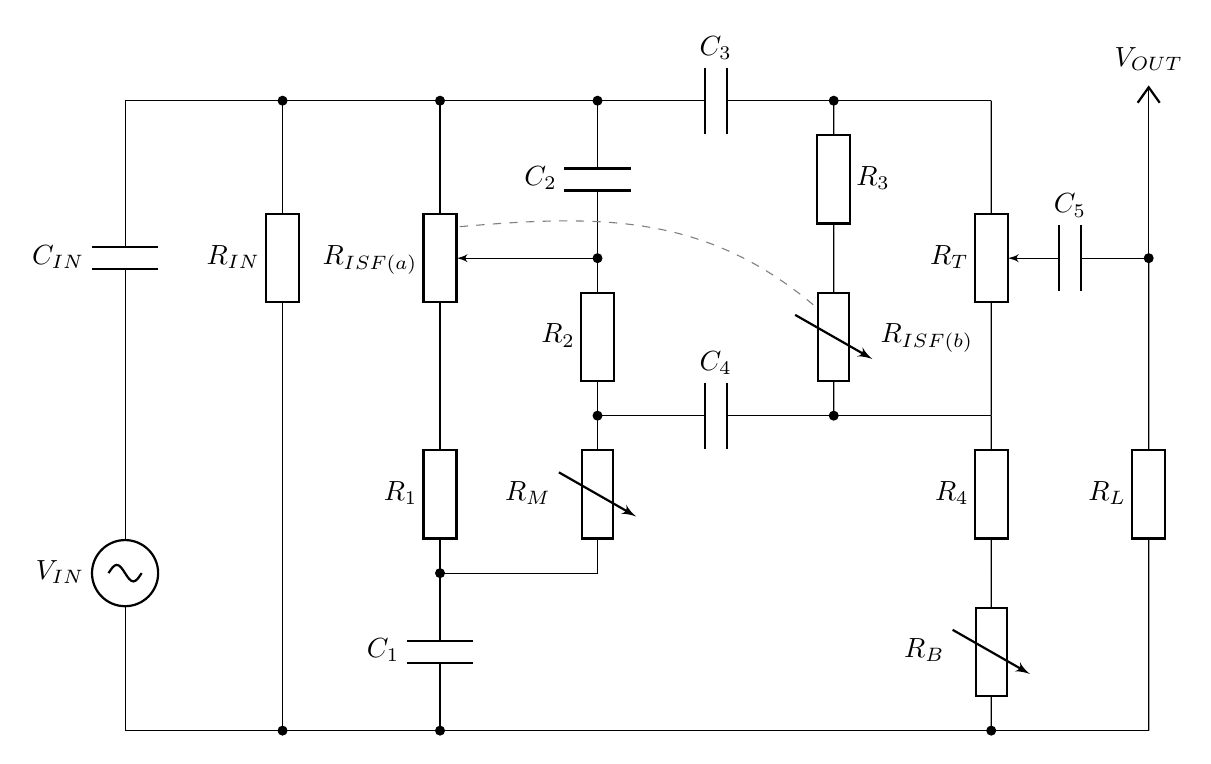
\begin{tikzpicture}
	\draw (2, 6) to[sinusoidal voltage source, l_=$V_{IN}$] (2, 2);

	\draw (4, 10) to[european resistor, l_=$R_{IN}$] (4, 6);
	\draw (6, 6) to[european resistor, l_=$R_1$] (6, 4);
	\draw (8, 8) to[european resistor, l_=$R_2$] (8, 6);
	\draw (11, 10) to[european resistor, l=$R_3$] (11, 8);
	\draw (13, 6) to[european resistor, l_=$R_4$] (13, 4);
	\draw (15, 8) to[european resistor, l_=$R_L$] (15, 2);

	\draw (13, 4) to[variable european resistor, l_=$R_B$] (13, 2);
	\draw (8, 6) to[variable european resistor, l_=$R_M$] (8, 4);
	\draw (13, 10) to[european potentiometer, l_=$R_T$] (13, 6);
	\draw (11, 8) to[variable european resistor, l=$R_{ISF(b)}$] (11, 6);
	\draw (6, 10) to[european potentiometer, l_=$R_{ISF(a)}$] (6, 6);

	\draw (2, 10) to[capacitor, l_=$C_{IN}$] (2, 6);
	\draw (6, 4) to[capacitor, l_=$C_1$] (6, 2);
	\draw (8, 10) to[capacitor, l_=$C_2$] (8, 8);
	\draw (8, 10) to[capacitor, l=$C_3$] (11, 10);
	\draw (8, 6) to[capacitor, l=$C_4$] (11, 6);
	\draw (13.5, 8) to[capacitor, l=$C_5$] (14.5, 8);

	\draw (8, 10) -- (2, 10);
	\draw (2, 2) -- (15, 2);
	\draw (4, 6) -- (4, 2);
	\draw (8, 4) -- (6, 4);
	\draw (6.56, 8) -- (8, 8);
	\draw (13, 10) -- (11, 10);
	\draw (11, 6) -- (13, 6);
	\draw (14.5, 8) -- (15, 8);
	\draw (15, 8) -- (15, 9.75);
	\draw[gray, dashed] (6.25, 8.4) to[out=5,in=140] (10.75, 7.4);

	\node[vcc] at (15, 9.75) {$V_{OUT}$};
	\node[circ] at (11, 10) {};
	\node[circ] at (11, 6) {};
	\node[circ] at (13, 2) {};
	\node[circ] at (15, 8) {};
	\node[circ] at (4, 10) {};
	\node[circ] at (4, 2) {};
	\node[circ] at (6, 10) {};
	\node[circ] at (6, 2) {};
	\node[circ] at (6, 4) {};
	\node[circ] at (8, 10) {};
	\node[circ] at (8, 6) {};
	\node[circ] at (8, 8) {};

\end{tikzpicture}
\end{document}